\begin{chapter}{Motivation and procedure for spawning wavepackets}
\label{ch:spawnprocedure}

In this chapter we will review the important parts from the paper about tunneling
dynamics and spawning \cite{GHJ_tunneling_spawning}. This is necessary because all
the further chapters about spawning of wavepackets in the non-adiabatic case build
upon and generalize the basic ideas developed there. Also we will work out the basic
mathematical procedure for spawning new wavepackets.


\section{The tunneling problem}

In tunneling dynamics we consider a potential shaped like a steep hill. The so
called Eckart potential, defined as $V\ofs{x} \assign \frac{v_0}{\cosh^2 \ofs{a x}}$
where $v_0$ is the potential energy at the maximum and $a$ is another constant,
serves as a good example of such a potential. This potential is shown in figure
\ref{fig:eckart_potential} for later reference.

\begin{figure}
  \centering
  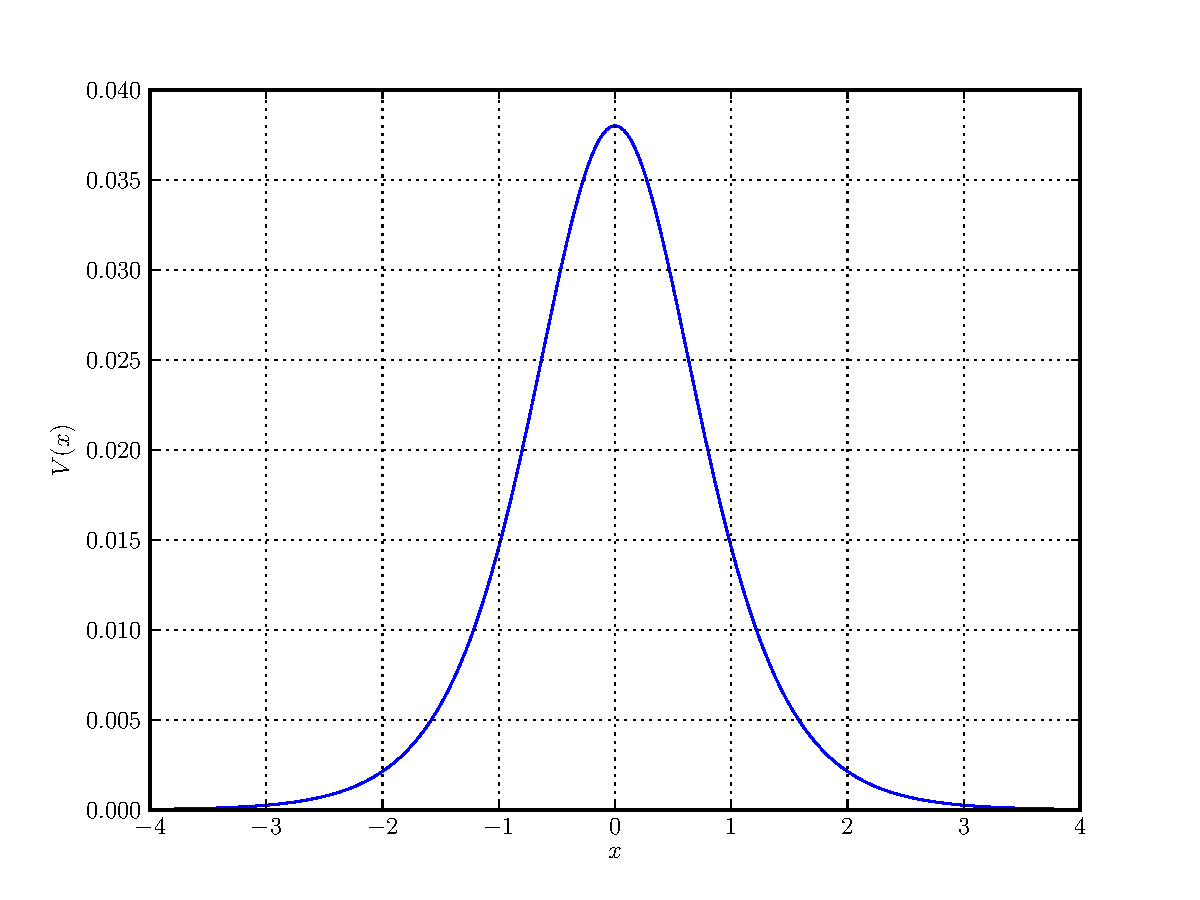
\includegraphics[scale=0.4]{./figures/eckart.pdf}
  \caption[The Eckart potential]{The Eckart potential with the parameters set to $v_0 = 0.038008$ and
  $a = 1.05836$ (same values as in ref.\cite{GHJ_tunneling_spawning}).}
  \label{fig:eckart_potential}
\end{figure}

Suppose now that we have a particle coming from one side and moving towards the
potential. In the classical world, the particle either crosses over the hill or
gets reflected depending on its momentum only. In the quantum world however, the
wavefunction always splits up in two parts of which one will be reflected and the
other transmitted. These two parts usually have very different amplitudes and will
drift apart more and more while their interaction rapidly becomes negligible as
they are separated by the potential hill.

\subsection{Motivation for spawning}

For our algorithm based on wavepackets as defined in chapter \ref{ch:wavepackets}
this split becomes problematical. The reason is that we need very high frequencies
to represent the tunneled part of our wavepacket. In most settings the energy of
the wavepacket is strictly smaller than the peak value of the potential. This implies
that during the propagation of the parameter set $\Pi$ the parameter $q$ which
centers the basis functions $\phi_k$ in position space gets reflected at the
potential. Therefore we get a good basis for representing the reflected part (with
only very few basis functions). This basis obviously is unsuitable for representing
the tunneled part and indeed we need many basis functions in the high frequency
domain. (These problems wouldn't matter if we worked with a infinite basis.)

In figure \ref{fig:tunneling_highfreq} the output of a tunneling simulation using
wavepackets is shown at late time. We clearly see the issue explained above. A basis
of size about $20$ would be sufficient for representing the reflected part accurately.
But for the transmitted part we need up to about $250$ basis functions. And the
problem gets worse with time (slowly) requiring more and more basis functions. Another important
point to notice is that there is a range of coefficients with negligible values in
the middle. In the example this range extends roughly from $40$ to $110$.

From this observation it's self-evident that breaking up the packet into two independent
parts would be a good idea. This then would also allow us to represent each packet
with a much smaller basis. And in the case of tunneling we could even neglect the
interaction between the two packets without loosing much information.

\begin{figure}
  \centering
  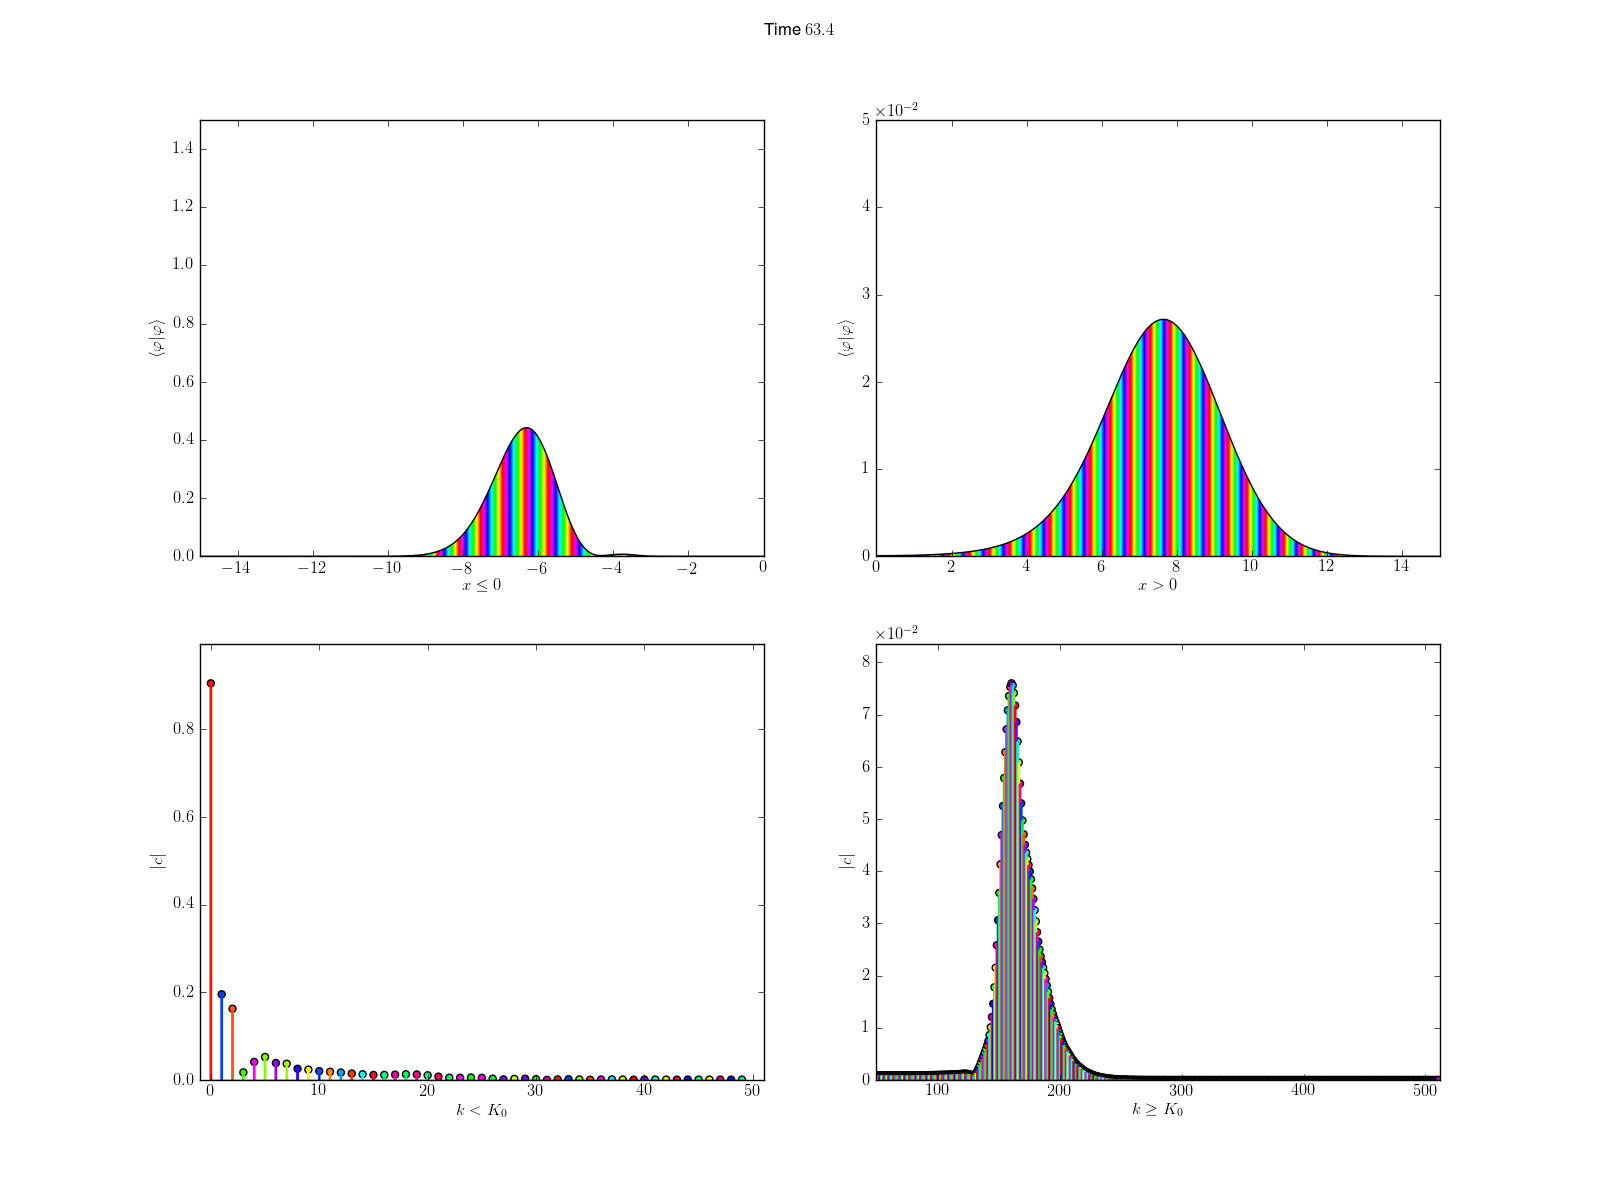
\includegraphics[width=\linewidth]{./figures/spawn_reason.png}
  \caption[Tunneling simulation example motivating the spawning approach]
  {This figure shows the output of a tunneling simulation at late time.
  The upper two panels show $\Braket{\Phi|\Phi}$ for the wavepacket $\Ket{\Phi}$.
  The lower two panels show the absolute value $|c_k|$ of the coefficients. The colors
  represent the complex phase according to the convention from \cite{Thaller_VQM}.
  Please notice the different scales! For the upper panels the $x$ axis is split
  at $0$ and the $y$ axes have a sensible scale. In the lower left panel we have
  the coefficients for $k < 50$ while the values for $k \geq 50$ are in the right
  panel where again the $y$ axis is scaled appropriately.}
  \label{fig:tunneling_highfreq}
\end{figure}


\section{Spawning a new packet}

With the motivation from the last section we will now investigate the steps that
have to be taken for spawning a new wavepacket. A first step is to find a new,
suitable basis. Remember that for fixed $\varepsilon$ the set of functions
$\{\phi_k\}_{k=0}^K$ gives a complete (but truncated) basis of the space $L^2$
and this is all we need for expanding our wavepacket into a linear combination.
Finding this basis is depicted in great detail in section \ref{sec:parameter_estimation}.
Although the mathematics behind this process is mostly trivial, there are plenty
of opportunities to make mistakes. Given this new basis we need to find a method
for transferring (a part of) the wavepacket to this new basis. We describe two
basically different methods in section \ref{sec:change_of_basis}.

\section{Parameter estimation}
\label{sec:parameter_estimation}

\subsection{Fragments}

In the remainder of this chapter we will use a so called \emph{fragment} $\Ket{w}$ as a
kind of a placeholder. The definition is very similar to the one of a full scalar
wavepacket $\Ket{\Phi}$ but more flexible for our purpose of lying out the basic
formalism for spawning wavepackets. So we define our fragment as

\begin{equation} \label{eq:def_fragment}
  \Ket{w} \assign \sum_{k=\alpha}^\beta c_k \phi_k
\end{equation}

with $\alpha, \beta \in \mathbb{N}_0$ and $\beta \geq \alpha$. Basically this is
just a handy abbreviation for an arbitrary linear combination of several basis functions.
If we demand that $\alpha,\beta \in \left[0, K-1\right]$ it becomes clear why we
call this a fragment, compared to the full (scalar) wavepacket in \eqref{eq:hawp_def_single}.
And in the case of $\alpha=0$ and $\beta=K-1$ we recover the full packet by

\begin{equation}
  \Ket{\Phi} = \exp\ofs{\frac{iS}{\varepsilon^2}} \Ket{w} \,.
\end{equation}

In principle the fragment could be sparse but this is mathematically equivalent
to saying that $\exists k \in \left[\alpha, \ldots, \beta\right] : c_k = 0$ and
thus we do not care further.

For the moment it does not matter what $w$ precisely is, all we need to know about
it is given by equation \eqref{eq:def_fragment}. Later $w$ may be a fully normalized
wavepacket $\Phi = \sum_{k=0}^{K-1} c_k \phi_k$, only a part of a wavepacket
$\Phi^\prime = \sum_{k=\alpha}^{\beta} c_k \phi_k$ with $\alpha \geq 0$ and
$\beta \leq K-1$ or a single component $\Phi_i = \sum_{k=0}^{K-1} c_k^i \phi_k^i$
of a homogeneous or inhomogeneous vector valued wavepacket $\Psi$ depending
on the context where the spawning technique is to be applied.  In the example
shown in figure \eqref{fig:tunneling_highfreq} motivating this chapter, $w$ would
be what is shown in the right column.

As said above the first step is to find a new (in some measure \emph{better})
basis $\{\tilde{\phi}_k\}_{k=0}^\infty$ of the space $L^2$ for representing $\Ket{w}$.
The basis functions $\tilde{\phi}_k$ are fully characterized by the parameter set
$\tilde{\Pi} \assign \{\tilde{P},\tilde{Q},\tilde{p},\tilde{q}\}$ so all we have
to do is estimate these four values. By the way, we denote all quantities in the
new bases with a tilde. The new position $\tilde{q}$ and new momentum $\tilde{p}$
are both real numbers and therefore easy. So we will handle these two first to
get a feeling for the procedure.


\subsection{Position $\tilde{q}$ and Momentum $\tilde{p}$}

The parameters $\tilde{q}$ and $\tilde{p}$ can be interpreted as the average position
and momentum. For this reason we compute expectation values of the position and momentum
operators

\begin{align}
  \tilde{q} & \assign \frac{\Braket{w | x | w}}{\Braket{w|w}} \\
  \tilde{p} & \assign \frac{\Braket{w | y | w}}{\Braket{w|w}}
\end{align}

where we divide by $\Braket{w|w}$ since the fragment is not normalized in general.
We can get an explicit expression for position operator $x$ and the momentum
operator $y$ by solving the linear system consisting of the definitions of both
ladder operators as shown in \eqref{eq:definition_ladder_ops} and get

\begin{equation}
\label{eq:definition_pos_and_mom_ops}
\begin{split}
  x \assign & \sqrt{\frac{\varepsilon^2}{2}} \left(Q \mathcal{R} + \conj{Q} \mathcal{L}\right) + q \\
  y \assign & \sqrt{\frac{\varepsilon^2}{2}} \left(P \mathcal{R} + \conj{P} \mathcal{L}\right) + p \,.
\end{split}
\end{equation}

Notice the symmetry in the two operators. We can transform $x$ into $y$ by the two
replacements $Q \rightarrow P$ and $q \rightarrow p$. This will halve the work
when calculating properties of these operators.

Starting with a fragment $\Ket{w}$ and an arbitrary operator $O$ and expanding the
linear combination we arrive at a double sum over brakets including basis functions
$\phi_k$ only

\begin{equation}
\label{eq:operator_expectation}
\begin{split}
  \Braket{w | O | w} \assign & \Braket{\sum_{k=\alpha}^\beta c_k \phi_k | O | \sum_{l=\alpha}^\beta c_l \phi_l} \\
                            = & \sum_{k=\alpha}^{\beta} \sum_{l=\alpha}^{\beta} \conj{c_k} c_l \Braket{\phi_k | O | \phi_l} \,.
\end{split}
\end{equation}

Now we have to see what happens with these simpler brakets. The full calculation
for the position operator $x$ works as follows where we use sesquilinearity and the
properties of the ladder operators

\begin{equation*}
\begin{split}
  \Braket{\phi_k | x | \phi_l}
  \assign & \Braket{\phi_k | \sqrt{\frac{\varepsilon^2}{2}} \left(Q \mathcal{R} + \conj{Q} \mathcal{L}\right) + q | \phi_l} \\
  = & \Braket{\phi_k | \sqrt{\frac{\varepsilon^2}{2}} Q \mathcal{R} | \phi_l}
    + \Braket{\phi_k | \sqrt{\frac{\varepsilon^2}{2}} \conj{Q} \mathcal{L} | \phi_l}
    + \Braket{\phi_k | q | \phi_l} \\
  = & \sqrt{\frac{\varepsilon^2}{2}} Q \Braket{\phi_k | \mathcal{R} | \phi_l}
    + \sqrt{\frac{\varepsilon^2}{2}} \conj{Q} \Braket{\phi_k | \mathcal{L} | \phi_l}
    + q \Braket{\phi_k | \phi_l} \\
  = & \sqrt{\frac{\varepsilon^2}{2}} Q \Braket{\phi_k | \sqrt{l+1} \phi_{l+1}}
    + \sqrt{\frac{\varepsilon^2}{2}} \conj{Q} \Braket{\phi_k | \sqrt{l} \phi_{l-1}}
    + q \Braket{\phi_k | \phi_l}
\end{split}
\end{equation*}

and finally we get

\begin{equation}
  \label{eq:estimate_pos_basis}
  \Braket{\phi_k | x | \phi_l}
  = \sqrt{\frac{\varepsilon^2}{2}} \left( Q \sqrt{l+1} \Braket{\phi_k | \phi_{l+1}}
    + \conj{Q} \sqrt{l} \Braket{\phi_k | \phi_{l-1}} \right)
    + q \Braket{\phi_k | \phi_l} \,.
\end{equation}

Applying the symmetry mentioned above we get a similar formula for the momentum
operator

\begin{equation}
  \label{eq:estimate_mom_basis}
  \Braket{\phi_k | y | \phi_l}
  = \sqrt{\frac{\varepsilon^2}{2}} \left( P \sqrt{l+1} \Braket{\phi_k | \phi_{l+1}}
    + \conj{P} \sqrt{l} \Braket{\phi_k | \phi_{l-1}} \right)
    + p \Braket{\phi_k | \phi_l} \,.
\end{equation}

Using the orthonormality of the basis function we can write

\begin{align}
  \Braket{\phi_k | x | \phi_l}
  & = \sqrt{\frac{\varepsilon^2}{2}} \left( Q \sqrt{l+1} \kron{k,l+1}
    + \conj{Q} \sqrt{l} \kron{k,l-1} \right)
    + q \kron{k,l} \\
  \Braket{\phi_k | y | \phi_l}
  & = \sqrt{\frac{\varepsilon^2}{2}} \left( P \sqrt{l+1} \kron{k,l+1}
    + \conj{P} \sqrt{l} \kron{k,l-1} \right)
    + p \kron{k,l} \,.
\end{align}

At this point we can substitute back these expressions into the double sum from
\eqref{eq:operator_expectation} which then gives

\begin{equation*}
\begin{split}
  \Braket{w | x | w} = & \sum_{k=\alpha}^\beta \sum_{l=\alpha}^\beta \conj{c_k} c_l
                         \left( \sqrt{\frac{\varepsilon^2}{2}} \left( Q \sqrt{l+1} \kron{k,l+1}
                         + \conj{Q} \sqrt{l} \kron{k,l-1} \right) + q \kron{k,l} \right) \\
  = &   \sum_{k=\alpha}^\beta \sum_{l=\alpha}^\beta \conj{c_k} c_l \sqrt{\frac{\varepsilon^2}{2}} Q \sqrt{l+1} \kron{k,l+1}
      + \sum_{k=\alpha}^\beta \sum_{l=\alpha}^\beta \conj{c_k} c_l \sqrt{\frac{\varepsilon^2}{2}} \conj{Q} \sqrt{l} \kron{k,l-1} \\
    & + \sum_{k=\alpha}^\beta \sum_{l=\alpha}^\beta \conj{c_k} c_l q \kron{k,l} \,.
\end{split}
\end{equation*}

Because of the Kronecker deltae each of these three double sums can be reduced
to a single sum only. For the first one we have $\kron{k,l+1} = 1 \iff l = k-1$
thus

\begin{equation} \label{eq:part1}
  \sum_{k=\alpha}^\beta \sum_{l=\alpha}^\beta \conj{c_k} c_l \sqrt{\frac{\varepsilon^2}{2}} Q \sqrt{l+1} \kron{k,l+1}
  = \sqrt{\frac{\varepsilon^2}{2}} Q \sum_{k=\alpha+1}^\beta \conj{c_k} c_{k-1} \sqrt{k} \,.
\end{equation}

See also figure \ref{fig:sumgrid} for a better overview over these nasty index transformations.
For the second sum the relation is $\kron{k,l-1} = 1 \iff l = k+1$ and therefore

\begin{equation} \label{eq:part2}
  \sum_{k=\alpha}^\beta \sum_{l=\alpha}^\beta \conj{c_k} c_l \sqrt{\frac{\varepsilon^2}{2}} \conj{Q} \sqrt{l} \kron{k,l-1}
  = \sqrt{\frac{\varepsilon^2}{2}} \conj{Q} \sum_{k=\alpha}^{\beta-1} \conj{c_k} c_{k+1} \sqrt{k+1} \,.
\end{equation}

The third one is trivial as $\kron{k,l} = 1 \iff l=k$ and we find

\begin{equation}
  \sum_{k=\alpha}^\beta \sum_{l=\alpha}^\beta \conj{c_k} c_l q \kron{k,l} = q \sum_{k=\alpha}^\beta \conj{c_k} c_k \,.
\end{equation}

Notice that this sum is nothing else than the norm of $w$.
We can simplify the expression for $\Braket{w|x|w}$ further. For this we first shift
the summation index of the right hand side of \eqref{eq:part2} up by one. (Equivalently
we could also shift down the index of \eqref{eq:part1} by one.) Mathematically this means
that $k^\prime = k+1$ which gives $k = k^\prime -1$ and we find that

\begin{equation} \label{eq:part2s}
  \sqrt{\frac{\varepsilon^2}{2}} \conj{Q} \sum_{k=\alpha}^{\beta-1} \conj{c_k} c_{k+1} \sqrt{k+1}
  = \sqrt{\frac{\varepsilon^2}{2}} \conj{Q} \sum_{k^\prime=\alpha+1}^{\beta} \conj{c_{k^\prime-1}} c_{k^\prime} \sqrt{k^\prime}
\end{equation}

where we wrote the primes once for clarity and drop them from now on. Recognizing
now that \eqref{eq:part1} and \eqref{eq:part2s} are complex conjugates of each other
we can combine them and write for the whole expression

\begin{align}
  \Braket{w|x|w}
  & = \sqrt{\frac{\varepsilon^2}{2}} Q \sum_{k=\alpha+1}^\beta \conj{c_k} c_{k-1} \sqrt{k}
    + \sqrt{\frac{\varepsilon^2}{2}} \conj{Q} \sum_{k=\alpha+1}^{\beta} \conj{c_{k-1}} c_{k} \sqrt{k}
    + q \sum_{k=\alpha}^\beta \conj{c_k} c_k \nonumber \\
  & = \sqrt{2 \varepsilon^2} \Re \left(Q \sum_{k=\alpha+1}^\beta \conj{c_k} c_{k-1} \sqrt{k} \right)
    + q \sum_{k=\alpha}^\beta \conj{c_k} c_k \,.
\end{align}

The very same procedure can be applied for the momentum operator $y$ too, but of
course we take the shortcut by symmetry and get

\begin{equation}
  \Braket{w|y|w}
  = \sqrt{2 \varepsilon^2} \Re \left(P \sum_{k=\alpha+1}^\beta \conj{c_k} c_{k-1} \sqrt{k} \right)
  + p \sum_{k=\alpha}^\beta \conj{c_k} c_k \,.
\end{equation}

If we now remember that the fragment may not be normalized we find the final formulae
for the expected position and momentum of $w$

\begin{align}
  \tilde{q} & \assign \frac{\Braket{w | x | w}}{\Braket{w|w}}
            = \frac{\sqrt{2 \varepsilon^2}}{\sum_{k=\alpha}^\beta \conj{c_k} c_k} \Re \left(Q \sum_{k=\alpha+1}^\beta \conj{c_k} c_{k-1} \sqrt{k} \right) + q 
            \label{eq:estimate_pos} \\
  \tilde{p} & \assign \frac{\Braket{w | y | w}}{\Braket{w|w}}
            = \frac{\sqrt{2 \varepsilon^2}}{\sum_{k=\alpha}^\beta \conj{c_k} c_k} \Re \left(P \sum_{k=\alpha+1}^\beta \conj{c_k} c_{k-1} \sqrt{k} \right) + p \,.
            \label{eq:estimate_mom}
\end{align}

\begin{figure}
  \centering
  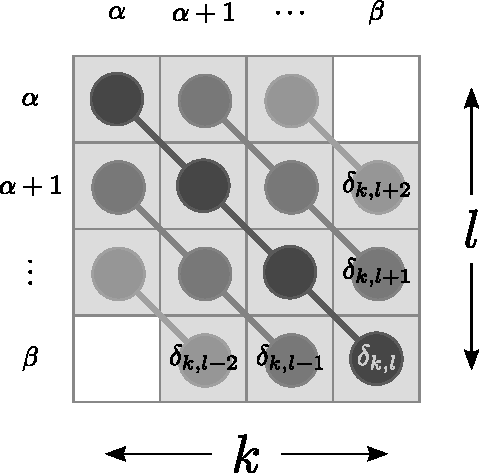
\includegraphics{./figures/sumgrid.pdf}
  \caption[Symbolic view on the double sum]{Symbolic view on the double sum
  $\sum_{k=\alpha}^\beta \sum_{l=\alpha}^\beta$. The diagonal lines show which
  elements remain in a single sum $\sum_k$ after expanding the corresponding
  Kronecker delta.}
  \label{fig:sumgrid}
\end{figure}

\subsection{Estimating second central moments}

In order to estimate the parameters $\tilde{Q}$ and $\tilde{P}$ of a fragment $w$
in a first step we have to compute the following two expectation values

\begin{equation} \label{eq:est_second_moments_def}
  \frac{\Braket{w | \left(x-\tilde{q}\right)^2 | w}}{\Braket{w|w}}
  \qquad \text{and} \qquad
  \frac{\Braket{w | \left(x-\tilde{p}\right)^2 | w}}{\Braket{w|w}}  
\end{equation}

which is in principle straight forward but very tedious. The reason why we compute
these quantities will become clear later but we essentially try to estimate second
central moments. We now show the whole procedure for the first braket and then use
the symmetry argument again to get the second one too. We start with expanding the
operator $\left(x-\tilde{q}\right)^2$ and break the expression into parts

\begin{equation} \label{eq:est_second_moment_pos}
\begin{split}
  \frac{\Braket{w | \left(x-\tilde{q}\right)^2 | w}}{\Braket{w|w}}
  & = \frac{\Braket{w | x^2 - 2 \tilde{q} x + \tilde{q}^2 | w}}{\Braket{w|w}} \\
  & = \frac{\Braket{w | x^2 | w}}{\Braket{w|w}}
    - 2 \tilde{q} \frac{\Braket{w | x | w}}{\Braket{w|w}}
    + \tilde{q}^2 \,.
\end{split}
\end{equation}

In the third term, the norms of $w$ cancel and we rediscover \eqref{eq:estimate_pos}
in  the second term. Thus all that is left over is

\begin{equation} \label{eq:est_second_moment_simplified}
  \frac{\Braket{w | \left(x-\tilde{q}\right)^2 | w}}{\Braket{w|w}}
  = \frac{\Braket{w | x^2 | w}}{\Braket{w|w}} - \tilde{q}^2 \,.
\end{equation}

Now we will concentrate on the first term and we have to struggle quite a bit to
compute it's numerator. As usual we decompose this braket by using the sesquilinearity
and write

\begin{equation} \label{eq:braket_basis_x2}
\begin{split}
  \Braket{w | x^2 | w}
  & = \Braket{\sum_{k=\alpha}^\beta c_k \phi_k | x^2 | \sum_{l=\alpha}^\beta c_l \phi_l} \\
  & = \sum_{k=\alpha}^\beta \sum_{l=\alpha}^\beta \conj{c_k} c_l \Braket{\phi_k | x^2 | \phi_l} \,.
\end{split}
\end{equation}

This reduced the problem to brakets over basis functions. At that point we need an
explicit version of the operator $x^2$ in terms of raising and lowering operators
which can be obtained as follows

\begin{equation} \label{eq:def_operator_x2}
\begin{split}
  x^2 & = \left(\sqrt{\frac{\varepsilon^2}{2}} \left(Q \mathcal{R} + \conj{Q} \mathcal{L}\right) + q\right)
          \left(\sqrt{\frac{\varepsilon^2}{2}} \left(Q \mathcal{R} + \conj{Q} \mathcal{L}\right) + q\right) \\
      & = \left( \theta Q \mathcal{R} + \theta \conj{Q} \mathcal{L} + q\right)
          \left( \theta Q \mathcal{R} + \theta \conj{Q} \mathcal{L} + q\right) \\
      & = \theta^2 Q\mathcal{R}Q\mathcal{R} + \theta^2Q\mathcal{R}\conj{Q}\mathcal{L}
        + \theta Q\mathcal{R}q + \theta^2 \conj{Q}\mathcal{L}Q\mathcal{R} + \theta^2\conj{Q}\mathcal{L}\conj{Q}\mathcal{L}
        + \theta \conj{Q}\mathcal{L}q + \theta qQ\mathcal{R} + \theta q \conj{Q}\mathcal{L} + q^2 \\
      & = \theta^2 Q^2 \mathcal{R}^2 + \theta^2 \conj{Q}^2 \mathcal{L}^2
        + \theta^2 Q\conj{Q} \mathcal{RL} + \theta^2 \conj{Q}Q \mathcal{LR}
        + 2\theta q Q \mathcal{R} + 2\theta q\conj{Q} \mathcal{L} + q^2
\end{split}
\end{equation}

where for simplicity we defined $\theta \assign \sqrt{\frac{\varepsilon^2}{2}}$.
We can now use the sesquilinearity of the inner product and split \eqref{eq:braket_basis_x2}
once more

\begin{align*}
  \Braket{\phi_k | x^2 | \phi_l} = & 
  \Braket{\phi_k | \theta^2 Q^2 \mathcal{R}^2 | \phi_l}
  +\Braket{\phi_k | \theta^2 \conj{Q}^2 \mathcal{L}^2 | \phi_l} \\
  & +\Braket{\phi_k | \theta^2 Q\conj{Q} \mathcal{RL} | \phi_l}
  +\Braket{\phi_k | \theta^2 \conj{Q}Q \mathcal{LR} | \phi_l} \\
  & +\Braket{\phi_k | 2\theta q Q \mathcal{R} | \phi_l}
  +\Braket{\phi_k | 2\theta q\conj{Q} \mathcal{L} | \phi_l}
  +\Braket{\phi_k | q^2 | \phi_l}
\end{align*}

resulting in seven parts which we will work out one after the other now. This is
a very boring task but necessary to justify the final relatively simple formula.

\begin{equation*}
\begin{split}
  \Braket{\phi_k | \theta^2 Q^2 \mathcal{R}^2 | \phi_l} & = \theta^2 Q^2 \Braket{\phi_k | \mathcal{R}^2 | \phi_l} \\
  & = \theta^2 Q^2 \Braket{\phi_k | \mathcal{R} | \sqrt{l+1} \phi_{l+1}} \\
  & = \theta^2 Q^2 \sqrt{l+1} \Braket{\phi_k | \sqrt{l+2} \phi_{l+2}} \\
  & = \theta^2 Q^2 \sqrt{l+1} \sqrt{l+2} \Braket{\phi_k | \phi_{l+2}}
    = \theta^2 Q^2 \sqrt{l+1} \sqrt{l+2} \kron{k,l+2}
\end{split}
\end{equation*}

\begin{equation*}
\begin{split}
  \Braket{\phi_k | \theta^2 \conj{Q}^2 \mathcal{L}^2 | \phi_l} & = \theta^2 \conj{Q}^2 \Braket{\phi_k | \mathcal{L}^2 | \phi_l} \\
  & = \theta^2 \conj{Q}^2 \Braket{\phi_k | \mathcal{L} | \sqrt{l} \phi_{l-1}} \\
  & = \theta^2 \conj{Q}^2 \sqrt{l} \Braket{\phi_k | \sqrt{l-1} \phi_{l-2}} \\
  & = \theta^2 \conj{Q}^2 \sqrt{l} \sqrt{l-1} \Braket{\phi_k | \phi_{l-2}}
    = \theta^2 \conj{Q}^2 \sqrt{l} \sqrt{l-1} \kron{k,l-2}
\end{split}
\end{equation*}

\begin{equation*}
\begin{split}
  \Braket{\phi_k | \theta^2 Q\conj{Q} \mathcal{RL} | \phi_l} & = \theta^2 Q\conj{Q} \Braket{\phi_k | \mathcal{RL} | \phi_l} \\
  & = \theta^2 Q\conj{Q} \Braket{\phi_k | \mathcal{R} | \sqrt{l} \phi_{l-1}} \\
  & = \theta^2 Q\conj{Q} \sqrt{l} \Braket{\phi_k | \sqrt{l} \phi_{l}} \\
  & = \theta^2 Q\conj{Q} l \Braket{\phi_k | \phi_{l}}
    = \theta^2 Q\conj{Q} l \kron{k,l}
\end{split}
\end{equation*}

\begin{equation*}
\begin{split}
  \Braket{\phi_k | \theta^2 \conj{Q}Q \mathcal{LR} | \phi_l} & = \theta^2 \conj{Q}Q \Braket{\phi_k | \mathcal{LR} | \phi_l} \\
  & = \theta^2 \conj{Q}Q \Braket{\phi_k | \mathcal{R} | \sqrt{l+1} \phi_{l+1}} \\
  & = \theta^2 \conj{Q}Q \sqrt{l+1} \Braket{\phi_k | \sqrt{l+1} \phi_{l}} \\
  & = \theta^2 \conj{Q}Q \left(l+1\right) \Braket{\phi_k | \phi_{l}}
    = \theta^2 \conj{Q}Q \left(l+1\right) \kron{k,l}
\end{split}
\end{equation*}

\begin{equation*}
\begin{split}
  \Braket{\phi_k | 2\theta qQ \mathcal{R} | \phi_l} & = 2\theta qQ \Braket{\phi_k | \mathcal{R} | \phi_l} \\
  & = 2\theta qQ \Braket{\phi_k | \sqrt{l+1} \phi_{l+1}} \\
  & = 2\theta qQ \sqrt{l+1} \Braket{\phi_k | \phi_{l+1}}
    = 2\theta qQ \sqrt{l+1} \kron{k,l+1}
\end{split}
\end{equation*}

\begin{equation*}
\begin{split}
  \Braket{\phi_k | 2\theta q\conj{Q} \mathcal{L} | \phi_l} & = 2\theta q\conj{Q} \Braket{\phi_k | \mathcal{L} | \phi_l} \\
  & = 2\theta q\conj{Q} \Braket{\phi_k | \sqrt{l} \phi_{l-1}} \\
  & = 2\theta q\conj{Q} \sqrt{l} \Braket{\phi_k | \phi_{l-1}}
    = 2\theta q\conj{Q} \sqrt{l} \kron{k,l-1}
\end{split}
\end{equation*}

\begin{equation*}
\begin{split}
  \Braket{\phi_k | q^2 | \phi_l} & = q^2 \Braket{\phi_k | \phi_l} = q^2 \kron{k,l}
\end{split}
\end{equation*}

Each time we used the properties of the ladder operators and the orthonormality
of the basis functions. With all these parts we are ready to take the pieces and
rebuild the original expression in bottom-up direction. The formula \eqref{eq:braket_basis_x2}
now becomes

\begin{equation} \label{eq:seven_double_sums}
\begin{split}
  \sum_{k=\alpha}^\beta \sum_{l=\alpha}^\beta \conj{c_k} c_l \Braket{\phi_k | x^2 | \phi_l} =
  & \sum_{k=\alpha}^\beta \sum_{l=\alpha}^\beta \conj{c_k} c_l \theta^2 Q^2 \sqrt{l+1} \sqrt{l+2} \kron{k,l+2}
    + \sum_{k=\alpha}^\beta \sum_{l=\alpha}^\beta \conj{c_k} c_l \theta^2 \conj{Q}^2 \sqrt{l} \sqrt{l-1} \kron{k,l-2} \\
  & + \sum_{k=\alpha}^\beta \sum_{l=\alpha}^\beta \conj{c_k} c_l \theta^2 Q\conj{Q} l \kron{k,l}
    + \sum_{k=\alpha}^\beta \sum_{l=\alpha}^\beta \conj{c_k} c_l \theta^2 \conj{Q}Q \left(l+1\right) \kron{k,l} \\
  & + \sum_{k=\alpha}^\beta \sum_{l=\alpha}^\beta \conj{c_k} c_l 2\theta qQ \sqrt{l+1} \kron{k,l+1}
    + \sum_{k=\alpha}^\beta \sum_{l=\alpha}^\beta \conj{c_k} c_l 2\theta q\conj{Q} \sqrt{l} \kron{k,l-1} \\
  & + \sum_{k=\alpha}^\beta \sum_{l=\alpha}^\beta \conj{c_k} c_l q^2 \kron{k,l} \,.
\end{split}
\end{equation}

Analogously to the last section all double sums collapse due to the Kronecker deltae.
The only tricky part is to get the summation limits right. It might help to keep
figure \ref{fig:sumgrid} in mind. Starting with the second off-diagonal terms (sums
1 and 2 in the above expression) we have that $\kron{k,l+2} = 1 \iff l=k-2$ and thus

\begin{equation} \label{eq:seven_double_sums_1}
  \sum_{k=\alpha}^\beta \sum_{l=\alpha}^\beta \conj{c_k} c_l \theta^2 Q^2 \sqrt{l+1} \sqrt{l+2} \kron{k,l+2}
  = \theta^2 Q^2 \sum_{k=\alpha+2}^\beta \conj{c_k} c_{k-2} \sqrt{k-1} \sqrt{k}
\end{equation}

and $\kron{k,l-2} = 1 \iff l=k+2$ causes

\begin{equation} \label{eq:seven_double_sums_2}
  \sum_{k=\alpha}^\beta \sum_{l=\alpha}^\beta \conj{c_k} c_l \theta^2 \conj{Q}^2 \sqrt{l} \sqrt{l-1} \kron{k,l-2}
  = \theta^2 \conj{Q}^2 \sum_{k=\alpha}^{\beta-2} \conj{c_k} c_{k+2} \sqrt{k+1}\sqrt{k+2} \,.
\end{equation}

With the first off-diagonal terms (sums 5 and 6 from above) we do the same. Because
$\kron{k,l+1} = 1 \iff l=k-1$ it holds that

\begin{equation} \label{eq:seven_double_sums_5}
  \sum_{k=\alpha}^\beta \sum_{l=\alpha}^\beta \conj{c_k} c_l 2\theta qQ \sqrt{l+1} \kron{k,l+1}
  = 2\theta qQ \sum_{k=\alpha+1}^\beta \conj{c_k} c_{k-1} \sqrt{k}
\end{equation}

and with $\kron{k,l-1} = 1 \iff l=k+1$ we get

\begin{equation} \label{eq:seven_double_sums_6}
  \sum_{k=\alpha}^\beta \sum_{l=\alpha}^\beta \conj{c_k} c_l 2\theta q\conj{Q} \sqrt{l} \kron{k,l-1}
  = 2\theta q\conj{Q} \sum_{k=\alpha}^{\beta-1} \conj{c_k} c_{k+1} \sqrt{k+1} \,.
\end{equation}

Finally for the diagonal terms (sums 3,4 and 7 from \eqref{eq:seven_double_sums})
we have trivially $\kron{k,l} = 1 \iff k=l$ giving

\begin{equation} \label{eq:seven_double_sums_34}
\begin{split}
  \sum_{k=\alpha}^\beta \sum_{l=\alpha}^\beta \conj{c_k} c_l \theta^2 Q\conj{Q} l \kron{k,l}
  & = \theta^2 Q\conj{Q} \sum_{k=\alpha}^\beta \conj{c_k} c_k k \\
  \sum_{k=\alpha}^\beta \sum_{l=\alpha}^\beta \conj{c_k} c_l \theta^2 \conj{Q}Q \left(l+1\right) \kron{k,l}
  & = \theta^2 \conj{Q}Q \sum_{k=\alpha}^\beta \conj{c_k} c_k \left(k+1\right)
\end{split}
\end{equation}

and

\begin{equation} \label{eq:seven_double_sums_7}
  \sum_{k=\alpha}^\beta \sum_{l=\alpha}^\beta \conj{c_k} c_l q^2 \kron{k,l}
  = q^2 \sum_{k=\alpha}^\beta \conj{c_k} c_k \,.
\end{equation}

The next step to proceed with is shifting the summation indices to a common base. For simplicity
we choose to shift down all sums to the starting point $\alpha$. The sum in \eqref{eq:seven_double_sums_5}
can be shifted by the index transformation $k^\prime = k-1$ and hence $k = k^\prime+1$
which when applied yields

\begin{equation} \label{eq:seven_double_sums_5s}
  2\theta qQ \sum_{k=\alpha+1}^\beta \conj{c_k} c_{k-1} \sqrt{k}
  = 2\theta qQ \sum_{k^\prime=\alpha}^{\beta-1} \conj{c_{k^\prime+1}} c_{k^\prime} \sqrt{k^\prime+1} \,.
\end{equation}

In the same fashion and be the transformation $k^\prime = k-2$ and hence $k = k^\prime+2$
we get for \eqref{eq:seven_double_sums_1}

\begin{equation} \label{eq:seven_double_sums_1s}
  \theta^2 Q^2 \sum_{k=\alpha+2}^\beta \conj{c_k} c_{k-2} \sqrt{k-1} \sqrt{k}
  = \theta^2 Q^2 \sum_{k^\prime=\alpha}^{\beta-2} \conj{c_{k^\prime+2}} c_{k^\prime} \sqrt{k^\prime+1} \sqrt{k^\prime+2} \,.
\end{equation}

Now that all summation indices are compatible we can combine some of these seven sums
and end up with less terms. The trick is again to recognize complex conjugate
pairs. The equations \eqref{eq:seven_double_sums_1s} and \eqref{eq:seven_double_sums_2}
are such a pair and we write

\begin{align} \label{eq:seven_double_sums_c12}
  \theta^2 Q^2 \sum_{k=\alpha}^{\beta-2} \conj{c_{k+2}} c_{k} \sqrt{k+1} \sqrt{k+2}
  \, + \, \theta^2 \conj{Q}^2 \sum_{k=\alpha}^{\beta-2} \conj{c_k} c_{k+2} \sqrt{k+1}\sqrt{k+2} \nonumber \\
  = 2 \theta^2 \Re \left( Q^2 \sum_{k=\alpha}^{\beta-2} \conj{c_{k+2}} c_{k} \sqrt{k+1} \sqrt{k+2} \right) \,.
\end{align}

In the same way we merge \eqref{eq:seven_double_sums_5s} and \eqref{eq:seven_double_sums_6}
into a single term

\begin{align} \label{eq:seven_double_sums_c56}
  2\theta qQ \sum_{k=\alpha}^{\beta-1} \conj{c_{k+1}} c_{k} \sqrt{k+1}
  \, + \, 2\theta q\conj{Q} \sum_{k=\alpha}^{\beta-1} \conj{c_k} c_{k+1} \sqrt{k+1} \nonumber \\
  = 4 \theta q \Re \left( Q \sum_{k=\alpha}^{\beta-1} \conj{c_{k+1}} c_{k} \sqrt{k+1} \right) \,.
\end{align}

Without any trick but simple algebra we can combine the two parts of \eqref{eq:seven_double_sums_34}
and get

\begin{equation} \label{eq:seven_double_sums_c34}
  \theta^2 Q\conj{Q} \sum_{k=\alpha}^\beta \conj{c_k} c_k k
  \, + \, \theta^2 \conj{Q}Q \sum_{k=\alpha}^\beta \conj{c_k} c_k \left(k+1\right)
  = \theta^2 Q\conj{Q} \sum_{k=\alpha}^\beta \conj{c_k} c_k \left(2k+1\right) \,.
\end{equation}

At the end of the day we can collect the remaining pieces \eqref{eq:seven_double_sums_c12},
\eqref{eq:seven_double_sums_c56}, \eqref{eq:seven_double_sums_c34} and \eqref{eq:seven_double_sums_7}
and rebuild the overall expression for $\Braket{w|x^2|w}$ as

\begin{equation} \label{eq:x2_braket}
\begin{split}
  \Braket{w|x^2|w}
  = & 2 \theta^2 \Re \left( Q^2 \sum_{k=\alpha}^{\beta-2} \conj{c_{k+2}} c_{k} \sqrt{k+1} \sqrt{k+2} \right) \\
  + & 4 \theta q \Re \left( Q \sum_{k=\alpha}^{\beta-1} \conj{c_{k+1}} c_{k} \sqrt{k+1} \right) \\
  + & \theta^2 Q\conj{Q} \sum_{k=\alpha}^\beta \conj{c_k} c_k \left(2k+1\right)
  + q^2 \sum_{k=\alpha}^\beta \conj{c_k} c_k \,.
\end{split}
\end{equation}

After we now finished the hardest part it is time to return the whole expression
\eqref{eq:est_second_moment_simplified} and we have all parts necessary to rewrite
this braket in terms of parameters sets $\Pi$, $\tilde{\Pi}$ and coefficients $c$
and $\varepsilon$ only. Define for the sake of readability

\begin{equation}
  W \assign \Braket{w|w} = \sum_{k=\alpha}^\beta \conj{c_k} c_k \,.
\end{equation}

and denote the first term in \eqref{eq:x2_braket} by $a$ and the third one by $c$.
Using these shortcuts we write

\begin{align*}
  \frac{\Braket{w|x^2|w}}{\Braket{w|w}} - \tilde{q}^2
  & = \frac{a + c}{W}
  + 2 q \frac{2\theta}{W} \Re \left( Q \sum_{k=\alpha}^{\beta-1} \conj{c_{k+1}} c_{k} \sqrt{k+1} \right)
  + q^2 - \tilde{q}^2
\intertext{and insert a decomposition of the zero}
  & = \frac{a + c}{W}
  + 2 q \frac{2\theta}{W} \Re \left( Q \sum_{k=\alpha}^{\beta-1} \conj{c_{k+1}} c_{k} \sqrt{k+1} \right) + 2 q^2 - 2q^2
  + q^2 - \tilde{q}^2 \\
  & = \frac{a + c}{W}
  + 2 q \left( \frac{2\theta}{W} \Re \left( Q \sum_{k=\alpha}^{\beta-1} \conj{c_{k+1}} c_{k} \sqrt{k+1} \right) + q \right)
  - q^2 - \tilde{q}^2
\intertext{where we find that the part inside the big parentheses is just $\tilde{q}$ and therefore we continue like}
  & = \frac{a + c}{W} + 2 q \tilde{q} - q^2 - \tilde{q}^2
\intertext{and factor the square}
  & = \frac{a + c}{W} - \left(q - \tilde{q}\right)^2 \,.
\end{align*}

We are left with second off-diagonal terms of $a$ and diagonal terms of $c$ only,
the first off-diagonal terms cancel respectively can be put inside the already
known value of $\tilde{q}$. To conclude this section we write the final formula

\begin{align} \label{eq:est_second_moment_pos_final}
  \frac{\Braket{w|\left(x-\tilde{q}\right)^2|w}}{\Braket{w|w}} & =
  \frac{
    \varepsilon^2 \Re \left( Q^2 \sum_{k=\alpha}^{\beta-2} \conj{c_{k+2}} c_{k} \sqrt{k^2+3k+2} \right) 
    + \frac{\varepsilon^2}{2} |Q|^2 \sum_{k=\alpha}^\beta \conj{c_k} c_k \left(2k+1\right)
  }{\sum_{k=\alpha}^\beta \conj{c_k} c_k}
  - \left(q - \tilde{q}\right)^2 \,.
\end{align}

Instead of repeating all this for the other braket $\Braket{w | \left(y-p\right)^2 | w}$
we apply the symmetry transformation here and replace \emph{every} $Q$ and $q$,
not only the ones that originally appear inside the operator $y$. This then yields

\begin{align} \label{eq:est_second_moment_mom_final}
  \frac{\Braket{w|\left(x-\tilde{p}\right)^2|w}}{\Braket{w|w}} & =
  \frac{
    \varepsilon^2 \Re \left( P^2 \sum_{k=\alpha}^{\beta-2} \conj{c_{k+2}} c_{k} \sqrt{k^2+3k+2} \right) 
    + \frac{\varepsilon^2}{2} |P|^2 \sum_{k=\alpha}^\beta \conj{c_k} c_k \left(2k+1\right)
  }{\sum_{k=\alpha}^\beta \conj{c_k} c_k}
  - \left(p - \tilde{p}\right)^2 \,.
\end{align}

If we have the case that the estimation of $\tilde{q}$ is perfect then the last
square vanishes. This really happens for the very specific special case where only
one of the coefficients is non-zero

\begin{equation*}
  c \assign \begin{pmatrix}
              c_\alpha = 0, \ldots, c_{\xi-1}=0, c_\xi=1, c_{\xi+1}=0, \ldots, c_{\beta} = 0
            \end{pmatrix}
    = \kron{k, \xi}
\end{equation*}

where $k$ is the index of a coefficient $c_k$. For computing the value of
$\Braket{w | x | w}$ we insert this Kronecker delta into the formula \eqref{eq:estimate_pos}

\begin{equation*}
\begin{split}
  \tilde{q} = \sqrt{2 \varepsilon^2} \Re \left(Q \sum_{k=\alpha+1}^\beta \conj{\kron{k,\xi}} \kron{k-1,\xi} \sqrt{k} \right) + q \,.
\end{split}
\end{equation*}

For a product of two Kronecker deltae it holds that

\begin{equation*}
  \kron{\alpha,\beta} \kron{\gamma,\delta} = 1 \quad \iff \quad \alpha = \beta \wedge \gamma = \delta \,.
\end{equation*}

Thus we get the unsatisfiable constraint that $k = \xi \wedge k-1 = \xi$ which
crunches the first sum to zero. What remains is

\begin{equation*}
  \tilde{q} = q \conj{c_\xi}c_\xi = q \,.
\end{equation*}

In the same way we get

\begin{equation*}
  \tilde{p} = p \,.
\end{equation*}

Note that these relations are \emph{not} true in general when we put no restrictions
on the coefficients $c$ of the fragment.


\subsection{Parameters $\tilde{P}$ and $\tilde{Q}$}
\label{sec:pq}

For the two parameters $\tilde{P}$ and $\tilde{Q}$ there is no trivial relation
as for $\tilde{p}$ and $\tilde{q}$, shown in formula \eqref{eq:estimate_pos} and \eqref{eq:estimate_mom}.
Computing the expectation value $\Braket{w|(x-\tilde{q})^2|w}$ is just the first
step on the way to $\tilde{P}$ and $\tilde{Q}$. The next step is given by the
relation which can be found at \cite[formula 2.24]{H_ladder_operators}. In our
notation for $P$ and $Q$ this translates to

\begin{equation}
  \Braket{\phi_k | \left(x-q\right)^2 | \phi_k} = \frac{\varepsilon^2}{2} |Q|^2 \left(2k + 1\right)
\end{equation}

and in analogy

\begin{equation}
  \Braket{\phi_k | \left(x-p\right)^2 | \phi_k} = \frac{\varepsilon^2}{2} |P|^2 \left(2k + 1\right) \,.
\end{equation}

Solving these equations for $|P|^2$ and $|Q|^2$ then gives

\begin{equation}
\label{eq:estimate_abssqrPQ}
\begin{split}
  |P|^2 & = \frac{2}{\varepsilon^2 \left(2k + 1\right)} \Braket{\phi_k | \left(x-p\right)^2 | \phi_k} \\
  |Q|^2 & = \frac{2}{\varepsilon^2 \left(2k + 1\right)} \Braket{\phi_k | \left(x-q\right)^2 | \phi_k} \,.
\end{split}
\end{equation}

We can then substitute the results from \eqref{eq:est_second_moment_pos_final} and
\eqref{eq:est_second_moment_mom_final} for the braket into this equation and get
and estimate of $|\tilde{Q}|^2$ and $|\tilde{P}|^2$. So this tells us how we
can estimate the squared absolute values of $\tilde{P}$ and $\tilde{Q}$ from
a fragment $w$ but not how to get the explicit complex values. A solution to this
dilemma was attempted in \cite[formula 16 and 17]{GHJ_tunneling_spawning} by
choosing $\tilde{Q}$ real and $\tilde{Q} > 0$ and then setting

\begin{equation}
\begin{split}
  \tilde{Q} & = \sqrt{|\tilde{Q}|^2} \\
  \tilde{P} & = \frac{\sqrt{\tilde{Q}^2 |\tilde{P}|^2-1}+i}{\tilde{Q}}
\end{split}
\end{equation}

but turned out to be incomplete in some situations. So we need to find a more
general solution. We know that $\tilde{P}$ and $\tilde{Q}$ are complex variables
hence we can decompose them as

\begin{equation}
\begin{split}
  \tilde{Q} & = a + ib \\
  \tilde{P} & = c + id \,.
\end{split}
\end{equation}

Denote the known values of $|\tilde{Q}|^2$ and $|\tilde{P}|^2$ by $v_{\tilde{Q}}$
and $v_{\tilde{P}}$. Of course the compatibility relations \eqref{eq:symplecticity_condition}
from chapter \ref{ch:wavepackets} still apply. Combining all these parts we
end up with the following system of equations

\begin{equation}
\begin{split}
  |\tilde{Q}|^2 & = v_{\tilde{Q}} \\
  |\tilde{P}|^2 & = v_{\tilde{P}} \\
  \conj{\tilde{Q}} \tilde{P} - \conj{\tilde{P}} \tilde{Q} & = 2i
\end{split}
\end{equation}

where we can plug in the explicit complex decomposition from above

\begin{equation}
\begin{split}
  a^2 + b^2 & = v_{\tilde{Q}} \\
  c^2 + d^2 & = v_{\tilde{P}} \\
  ad - bc -1 & = 0 \,.
\end{split}
\end{equation}

We have only three equations for the four variables $a, b, c \text{ and } d \in \mathbb{R}$
so there is one degree of freedom in these expressions. In principle we could read
the restriction from above and use $b=0$ as a fourth equation. But even with this
restriction the system has four solutions because of the multivalued nature of the
square root function

\begin{subequations} \label{eq:pq_possibilities}
\begin{align}
  \tilde{Q} & = -\sqrt{v_{\tilde{Q}}} & \tilde{P} & = -\sqrt{v_{\tilde{P}}-\frac{1}{v_{\tilde{Q}}}}-\frac{i}{\sqrt{v_{\tilde{Q}}}} \\
  \tilde{Q} & =  \sqrt{v_{\tilde{Q}}} & \tilde{P} & = -\sqrt{v_{\tilde{P}}-\frac{1}{v_{\tilde{Q}}}}+\frac{i}{\sqrt{v_{\tilde{Q}}}} \\
  \tilde{Q} & = -\sqrt{v_{\tilde{Q}}} & \tilde{P} & =  \sqrt{v_{\tilde{P}}-\frac{1}{v_{\tilde{Q}}}}-\frac{i}{\sqrt{v_{\tilde{Q}}}} \\
  \tilde{Q} & =  \sqrt{v_{\tilde{Q}}} & \tilde{P} & =  \sqrt{v_{\tilde{P}}-\frac{1}{v_{\tilde{Q}}}}+\frac{i}{\sqrt{v_{\tilde{Q}}}} \,. 
\end{align}
\end{subequations}
  
Therefore we need a criterion to choose one of these solutions. But let us first
go on in the spawning procedure and assume for now that we have a valid value
for $\tilde{Q}$ and $\tilde{P}$.


\subsection{Algorithmic formulation of parameter estimation}

The algorithm \ref{al:parameter_estimation} summarizes the steps shown in the last
sections. Given a fragment $w$ together with all necessary information it will
compute a new parameter set $\tilde{\Pi}$ and hence a new basis of $L^2$. This
is the last step to take before we can go on and move the fragment $w$ into
this new basis.

\begin{algorithm}
\caption{Parameter estimation for fragments}
\label{al:parameter_estimation}
\begin{algorithmic}
  \REQUIRE The parameters $\Pi$ of the fragment $w$
  \REQUIRE The coefficients $\{c_i\}_{i=\alpha}^{\beta}$ of the fragment $w$
  \REQUIRE $\alpha \geq 0$ and $\beta \leq K-1$
  \REQUIRE A value for $k \in \{0, \ldots, \eta-1\}$
  \STATE // Compute the squared norm of $w$
  \STATE $\|w\|^2 \assign \sum_{k=\alpha}^\beta \conj{c_k} c_k$
  \STATE // Compute the expectations for position and momentum
  \STATE $\vartheta_0 \assign \sum_{k=\alpha+1}^\beta \conj{c_k} c_{k-1} \sqrt{k}$
  \STATE $\tilde{q} \assign \frac{\sqrt{2 \varepsilon^2}}{\|w\|^2} \Re \left(Q \vartheta_0 \right) + q$
  \STATE $\tilde{p} \assign \frac{\sqrt{2 \varepsilon^2}}{\|w\|^2} \Re \left(P \vartheta_0 \right) + p$
  \STATE // Estimate second moments
  \STATE $\vartheta_1 \assign \sum_{k=\alpha}^{\beta-2} \conj{c_{k+2}} c_{k} \sqrt{k^2+3k+2}$
  \STATE $\vartheta_2 \assign \sum_{k=\alpha}^\beta \conj{c_k} c_k \left(2k+1\right)$
  \STATE $M_{\tilde{Q}} \assign \frac{\varepsilon^2}{\|w\|^2} \left(
          \Re \left( Q^2 \vartheta_1 \right) + \frac{1}{2} |Q|^2 \vartheta_2 \right)
          - \left(q - \tilde{q}\right)^2$
  \STATE $M_{\tilde{P}} \assign \frac{\varepsilon^2}{\|w\|^2} \left(
          \Re \left( P^2 \vartheta_1 \right) + \frac{1}{2} |P|^2 \vartheta_2 \right)
          - \left(p - \tilde{p}\right)^2$
  \STATE // Plug into \eqref{eq:estimate_abssqrPQ}
  \STATE $|\tilde{Q}|^2 \assign \frac{2}{\varepsilon^2 \left(2k + 1\right)} M_{\tilde{Q}} $
  \STATE $|\tilde{P}|^2 \assign \frac{2}{\varepsilon^2 \left(2k + 1\right)} M_{\tilde{P}} $
  \STATE // The set of new parameters 
  \STATE $\tilde{\Pi} \assign \{\tilde{P}, \tilde{Q}, S, \tilde{p}, \tilde{q}\}$
  \RETURN $\tilde{\Pi}$
\end{algorithmic}
\end{algorithm}


\section{Change of basis}
\label{sec:change_of_basis}

The second step in the spawning process is a simple change of basis. Under this
term we summarize several methods. Not all of them correspond to what is a change
of basis in the sense of linear algebra. We have computed another basis of $L^2$
in the last sections by finding a new set of parameters $\tilde{\Pi}$. This establishes
a new basis $\{\tilde{\phi}_k\}_k$ that we will use for representing the spawned
fragment $\Ket{\tilde{w}}$. 

The mathematical formulation of the problem we want to solve in this section can
be posed as: \emph{given a fragment $w$ by}

\begin{equation}
  w = \sum_{k=\alpha}^{\beta} c_k \phi_k
\end{equation}

\emph{in the old basis, find new coefficients $\left(d_0, \ldots, d_{\eta}\right)$ such
that $w$ can be written as a linear combination in the new basis}

\begin{equation}
  w \approx \tilde{w} \assign \sum_{k=0}^{\eta} d_k \tilde{\phi_k}
\end{equation}

\emph{with conserving $\|w + \tilde{w}\|$ as much as possible.} With an
infinite basis, i.e. $\eta=\infty$ we could achieve a perfect transformation in
all cases and hence an equal sign in the equation above.

Throughout this section we will assume that the original basis is of size $K$
and the set of coefficients of the basis expansion is denoted by
$c \assign \{c_k\}_{k=0}^{K-1}$. For the fragment $w$ we require that $\alpha \geq 0$
and $\beta \leq K-1$. The new basis can have a different size $\eta$ which we usually
choose much smaller than $K$ and we call the set of new coefficients $d \assign \{d_k\}_{k=0}^{\eta-1}$.


\subsection{Lumping procedure}

A very simple way to find the coefficients $d$ is what we call the \emph{lumping method}.
The method can be explained best if we assume for the moment that we want to spawn
a single Gaussian $\phi_0$ only. This assumption then gives a first hint that all
$d_k$ with $k>0$ are set to zero and we only have to find a value for $d_0$. Since
there has to be norm conservation of $w + \tilde{w}$ with initially $\|\tilde{w}\| = 0$
and after spawning $\|w\| = 0$ we have to set

\begin{equation}
  d_0 \assign \|w\| \,.
\end{equation}

But we also have to remove the fragment  $w$ and set $c_\alpha, \ldots c_\beta$
to zero. Therefore we can summarize the whole procedure by the following two
assignments

\begin{equation}
\begin{split}
  \begin{pmatrix}
    c_\alpha & \cdots & c_\beta
  \end{pmatrix} & \assign 0 \\
  d & \assign
  \begin{pmatrix}
    d_0 & 0 & \cdots & 0
  \end{pmatrix}
\end{split}
\end{equation}

where $d_0 = \sqrt{\Braket{w,w}} = \|w\|$ and all other coefficients up to $d_\eta$
are 0. With this method we get perfect norm conservation but this does not imply
perfect approximation or minimal spawning error and $\|w - \tilde{w}\| \neq 0$ in
general because $w$ is not a Gaussian in general. When applying this method to
tunneling problems, $w$ is a Gaussian at least asymptotically and the method is
therefore appropriate. The details can be found in reference \cite{GHJ_tunneling_spawning}.

If we a priori know what value $k$ will have or in other words which basis function
$\tilde{\phi}_k$ will dominate then we can take this into account and set $d_k = \|w\|$
and $d_i = 0$ for all $i \neq k$. The algorithm \ref{al:lumping_method} shows
again the precise details of this method.

\begin{algorithm}
\caption{Lumping method for the change of basis}
\label{al:lumping_method}
\begin{algorithmic}
  \REQUIRE The size $K$ of the old and $\eta$ of the new basis
  \REQUIRE The fragment $w$ with its coefficients $\{c_i\}_{i=\alpha}^{\beta}$
  \REQUIRE $\alpha \geq 0$ and $\beta \leq K-1$
  \REQUIRE A value for $k \in \{0, \ldots, \eta-1\}$
  \STATE // Initialize all new coefficients with zero
  \STATE $\left(d_0, \ldots, d_{\eta}\right) \assign 0$
  \STATE // Assign the norm of $w$ to the new coefficient $k$
  \STATE $d_k \assign \sqrt{\sum_{i=\alpha}^\beta c_i^2}$
  \STATE // Set the old coefficients to zero
  \STATE $\left(c_\alpha, \ldots, c_\beta\right) \assign 0$
  \RETURN $d = \left(d_0, \ldots, d_{\eta}\right)$
\end{algorithmic}
\end{algorithm}

A more general version of the lumping method would use the first $\mu$ coefficients
$d_0, \ldots, d_{\mu-1}$ and hence effectively spawn a linear combination instead of
a pure single basis function $\tilde{\phi_k}$ but in that case it is not obvious
what values have to be given to these $\{d_i\}_{i=0}^{\mu-1}$.

\subsection{Basis projection procedure}

Another method for the change of basis is called the \emph{basis projection} and is
a real projection in the sense of linear algebra. The task now requires projecting $w$
to the new basis specified by the parameter set $\tilde{\Pi}$ and consisting of
basis functions $\{\tilde{\phi}_k\}_{k=0}^{\eta-1}$. We can derive the following
projection formula for the coefficients $d_i$ of the spawned fragment $\tilde{w}$ by
using the normed inner product

\begin{equation} \label{eq:basis_projection}
  d_i \assign \frac{\Braket{w|\tilde{\phi}_i}}{\Braket{w|w}} \,.
\end{equation}

The inner product above is essentially an integral, so we can apply our quadrature
rule $\left(\gamma, \omega\right)$ of order $R$ here and get

\begin{equation} \label{eq:projection_quadrature}
  d_i = \varepsilon \cdot Q_0 \sum_{r=0}^{R-1} \conj{w\ofs{\gamma_r}} \cdot \tilde{\phi}_i \ofs{\gamma_r} \cdot \omega_r \,.
\end{equation}

If we write out the $w\ofs{\gamma_r}$ part as basis expansion we get the following
relation which now can be computed directly

\begin{equation} \label{eq:projection_quadrature_full}
  d_i = \varepsilon \cdot Q_0 \sum_{r=0}^{R-1} \conj{\sum_{k=\alpha}^\beta c_k \phi_k\ofs{\gamma_r}} \cdot \tilde{\phi}_i \ofs{\gamma_r} \cdot \omega_r \,.
\end{equation}

We repeat the above quadrature for each $i$ in the range $\{0, \ldots, \mu-1\}$
where $\mu < \eta$ and hence projecting on the first $\mu$ basis functions
$\{\tilde{\phi}_k\}_{k=0}^{\mu-1}$ of the spawned basis. From this projection we
get the non-zero coefficients $\{d_i\}_{i=0}^{\mu-1}$ of the new fragment $\tilde{w}$
while all higher $d_i$ with $i \geq \mu$ are zero. At this moment we have to
remove the part of $w$ and set the coefficients $c_\alpha, \ldots, c_\beta$
to zero. The following two assignments give an overview over both operations

\begin{equation}
\begin{split}
  d & \assign
  \begin{pmatrix}
    d_0 & \cdots & d_{\mu} & d_{\mu+1} = 0 & \cdots & d_{\eta-1} = 0
  \end{pmatrix} \\
  \begin{pmatrix}
    c_\alpha & \cdots & c_\beta
  \end{pmatrix} & \assign 0 \,.
\end{split}
\end{equation}

If we want to spawn only a single Gaussian then we can simply set $\mu$ to $0$
but projecting only onto $\tilde{\phi}_0$ is not the same as lumping with $k=0$.
When $\eta$ is really small for example say below 8 then we project on a very
small basis and might loose much of the norm of $w$, thus it can happen that
$\|\tilde{w}\| \ll \|w\|$. This is the case when $w$ has only minor components
in the direction of the first $\mu$ new basis functions. In contrast to this we
have perfect norm conservation with lumping. On the other hand, spawning whole
linear combinations here arises naturally from the projection while it's a currently
unsolved problem with the lumping method. In general the projection method with
a sensible size $\eta$ of the basis will give better results than lumping as
in most simulations we will never have pure basis states and this is the only
case where lumping is really advantageous.

The only remaining question now is which rule we use for the quadrature in
\eqref{eq:projection_quadrature_full}. There are at least three reasonable options
and it's not entirely clear yet which is the best one. Mathematically the
mixing quadrature from section \ref{sec:mixing_quadrature} is the only correct choice.
The mixing quadrature is considered to be correct because $w$ in the bra and the $\tilde{\phi}_i$
in the ket belong to two different bases with parameters sets $\Pi$ and $\tilde{\Pi}$
respectively thus we have to mix the two sets as shown in algorithm \ref{al:mixing_hagedorn_parameters}
for a good quadrature. But we may also want to focus the quadrature rule onto
the spawned wavepacket $\tilde{w}$. This seems to be also a good idea at first
glance because we are interested in the projection of $w$ to the new basis given
by $\tilde{\Pi}$. But it turns out that this focusing yields a worse norm
conservation than mixing quadrature, compare the panels in figure \ref{fig:quadrature_choice}
for an explicit example. For this reason we concentrate only on the mixing quadrature.

\begin{figure}
  \centering
  \subfloat[][]{
    \label{fig:quad_mother}
    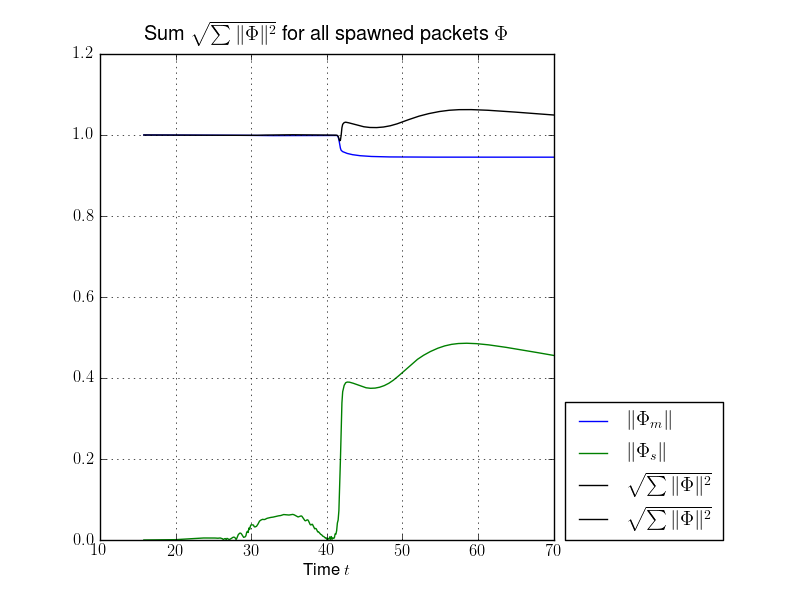
\includegraphics[width=0.5\linewidth]{./figures/norms_quad_mother.png}
  }
  \subfloat[][]{
    \label{fig:quad_drift_mother}
    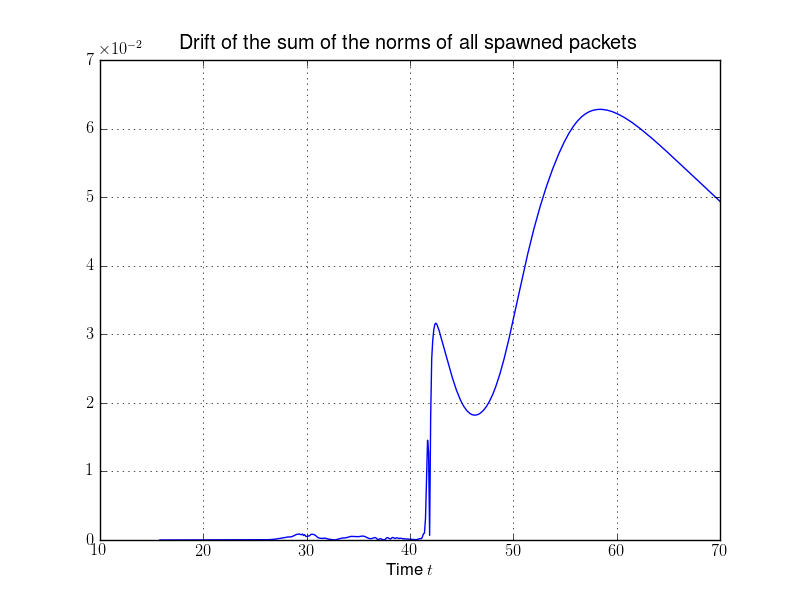
\includegraphics[width=0.5\linewidth]{./figures/norms_drift_quad_mother.png}
  } \\
  \subfloat[][]{
    \label{fig:quad_child}
    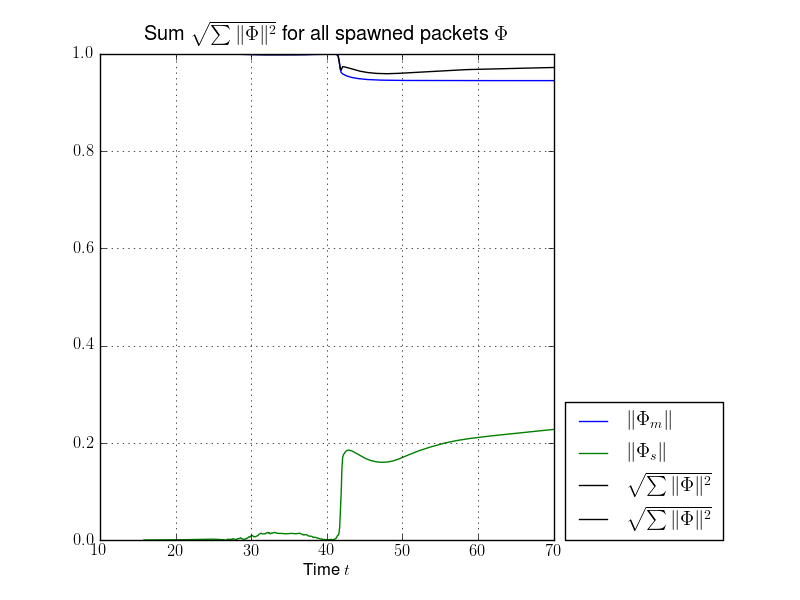
\includegraphics[width=0.5\linewidth]{./figures/norms_quad_child.png}
  }
  \subfloat[][]{
    \label{fig:quad_drift_child}
    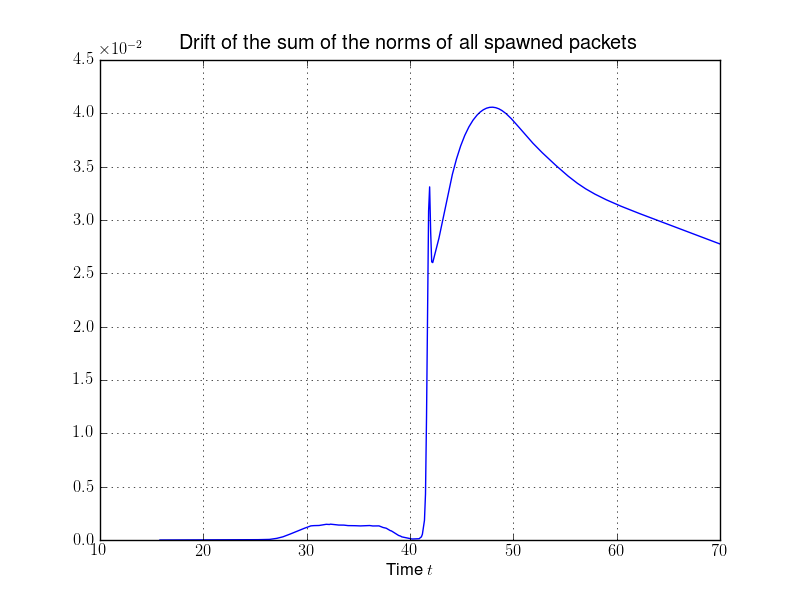
\includegraphics[width=0.5\linewidth]{./figures/norms_drift_quad_child.png}
  } \\
  \subfloat[][]{
    \label{fig:quad_mix}
    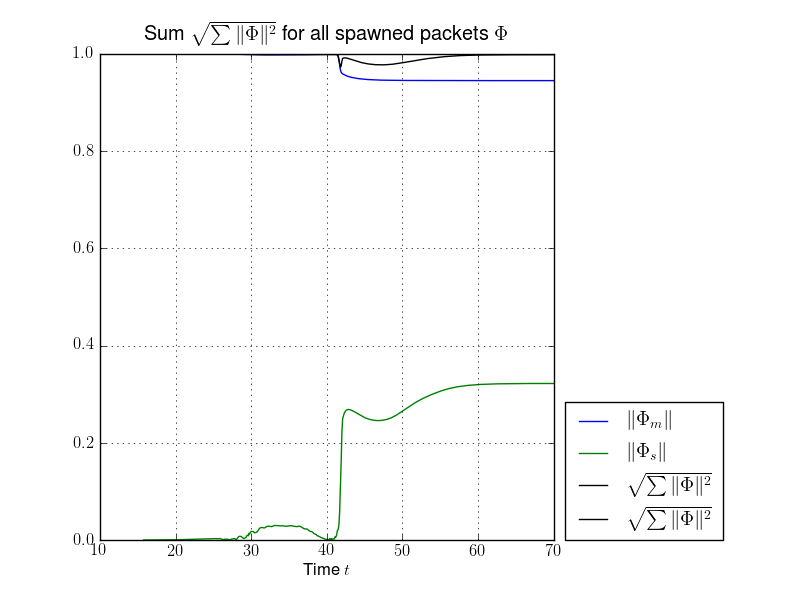
\includegraphics[width=0.5\linewidth]{./figures/norms_quad_mix.png}
  }
  \subfloat[][]{
    \label{fig:quad_drift_mix}
    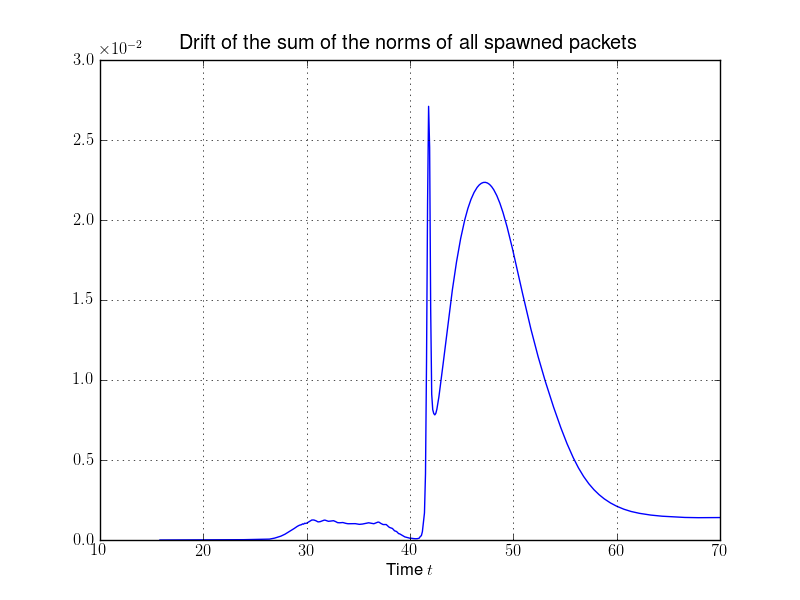
\includegraphics[width=0.5\linewidth]{./figures/norms_drift_quad_mix.png}
  } \\
  \caption[Comparison of quadratures used for basis projection]{
  The plots show the norms and the norm drift obtained by spawning with
  the projection method. For the quadrature used inside the projection method there
  are three possibilities: the quadrature can be homogeneous and focused on either
  the mother or the child (spawned) wavepacket. Or it can be the fully inhomogeneous
  quadrature, which is the only correct choice from the mathematical point of
  view and also yields the least and most rapidly decaying error.
  \subref{fig:quad_mother} Norm, computed with quadrature focused on the mother part.
  \subref{fig:quad_drift_mother} Difference to the theoretical norm, computed with quadrature focused on the mother part.
  \subref{fig:quad_child} Norm, computed with quadrature focused on the child part.
  \subref{fig:quad_drift_child} Difference to the theoretical norm, computed with quadrature focused on the child part.
  \subref{fig:quad_mix} Norm, computed with inhomogeneous quadrature.
  \subref{fig:quad_drift_mix} Difference to the theoretical norm, computed with inhomogeneous quadrature.
  \label{fig:quadrature_choice}
  }
\end{figure}

Algorithm \ref{al:projection_method} shows an algorithmic formulation of basis
projection method. The code is inefficient because of the nested loops and the
actual implementation uses several optimizations like vectorization and contains
no explicit loop.

\begin{algorithm}
\caption{Basis projection method for the change of basis}
\label{al:projection_method}
\begin{algorithmic}
  \REQUIRE The size $K$ of the old and $\eta$ of the new basis
  \REQUIRE The parameters $\Pi$ and $\tilde{\Pi}$ defining the bases
  \REQUIRE The two sets of basis functions $\{\phi_k\}_{k=0}^{K-1}$ and $\{\tilde{\phi}_k\}_{k=0}^{\eta-1}$
  \REQUIRE The mother fragment $w$ with its coefficients $\{c_k\}_{k=\alpha}^{\beta}$
  \REQUIRE A mixing quadrature rule of order $R$ with nodes $\gamma$ and weights $\omega$
  \REQUIRE A value for $\mu \in \{0, \ldots, \eta-1\}$
  \REQUIRE $\alpha \geq 0$ and $\beta \leq K-1$

  \STATE // Compute $Q_S$ from mixing $\Pi$ and $\tilde{\Pi}$ by the mixing procedure \ref{al:mixing_hagedorn_parameters}
  \STATE $Q_S \assign \text{mix\_parameters}(\Pi, \tilde{\Pi})$

  \STATE // Initialize all new coefficients with zero
  \STATE $\left(d_0, \ldots, d_{\eta-1}\right) \assign 0$

  \STATE // Project to the basis of the spawned part and compute new coefficients

  \FOR{$i \assign 0$ \TO $\mu$}
    \FOR{$r \assign 0$ \TO $R-1$}
      \STATE $d_i \assign d_i + \conj{  \sum_{k=\alpha}^\beta c_k \phi_k\ofs{\gamma_r}} \cdot \tilde{\phi}_i \ofs{\gamma_r} \cdot \omega_r$
    \ENDFOR
    \STATE $d_i \assign \varepsilon \cdot Q_S \cdot d_i$
  \ENDFOR

  \STATE // Set the old coefficients to zero
  \STATE $\left(c_\alpha, \ldots, c_\beta\right) \assign 0$

  \RETURN $d \assign \left(d_0, \ldots, d_{\eta-1}\right)$
\end{algorithmic}
\end{algorithm}


\section{Problematic difficulties and open issues}

Now we can return to the problem of choosing concrete values for $\tilde{P}$ and $\tilde{Q}$
we deferred at the end of section \ref{sec:pq}. After we developed the formalism
to really create the spawned fragments $\tilde{w}$ in the last section we can
now use this to determine the best choice among the four possibilities of \eqref{eq:pq_possibilities}.
The idea is to spawn a fragment using each of these four different parameter pairs
resulting in the test fragments $\tilde{w_1}, \tilde{w_2}, \tilde{w_3} \text{ and } \tilde{w_4}$.
And then we can try to maximize the overlap with the original fragment $w$

\begin{equation}
  \arg \max_i \Braket{\tilde{w_i}|w} \,.
\end{equation}

This gives us then the best pair of parameters and we can finish the set $\tilde{\Pi}$.
The drawback of this method is that while the original parameters $P\ofs{t}$ and
$Q\ofs{t}$ are continuous and smooth functions of time, this maximization procedure
can introduce arbitrary jumps. Hence while this method works most of the time
and these jumps do not matter for our purposes it's still not the optimal solution.
When we combine spawning and propagation later these jumps won't be a problem
because we spawn once and the propagate smoothly.

~\newline

Another severe problem already mentioned above is posed by the $k$ in formula
\eqref{eq:estimate_abssqrPQ}. In general we do not work with single basis functions
but with fragments which are linear combinations thereof. Therefore we need to
estimate the parameters for such a linear combination to get a good basis for spawning.
We have no way to know a value of $k$ at spawning time and we also have no suitable
way to compute it. For the tunneling problem it can be shown \cite{GHJ_exponentially_accurate}
that the transmitted part is always a Gaussian (at least asymptotically for large times)
and hence we can set $k=0$ there and spawn a $\phi_0$ by lumping. (The procedure
still works for the basis projection method, but depends on the fact that
we can set $k=0$ as justified by theory.) More on this in the next chapter.

In the non-adiabatic case $k$ can have any value. Additionally we won't spawn
just a single function $\phi_k$ but a whole linear combination $\sum_i \phi_i$.
Under these circumstances it is even more obscure what $k$ should be. A real world
example is shown in figure \ref{fig:spawn_issues_k_na} where we would like to
spawn on the lower level. The fragment there has clearly the shape of a $\phi_2$
but setting $k=2$ can not be justified if we look at the lower right panel.

\begin{figure}
  \centering
  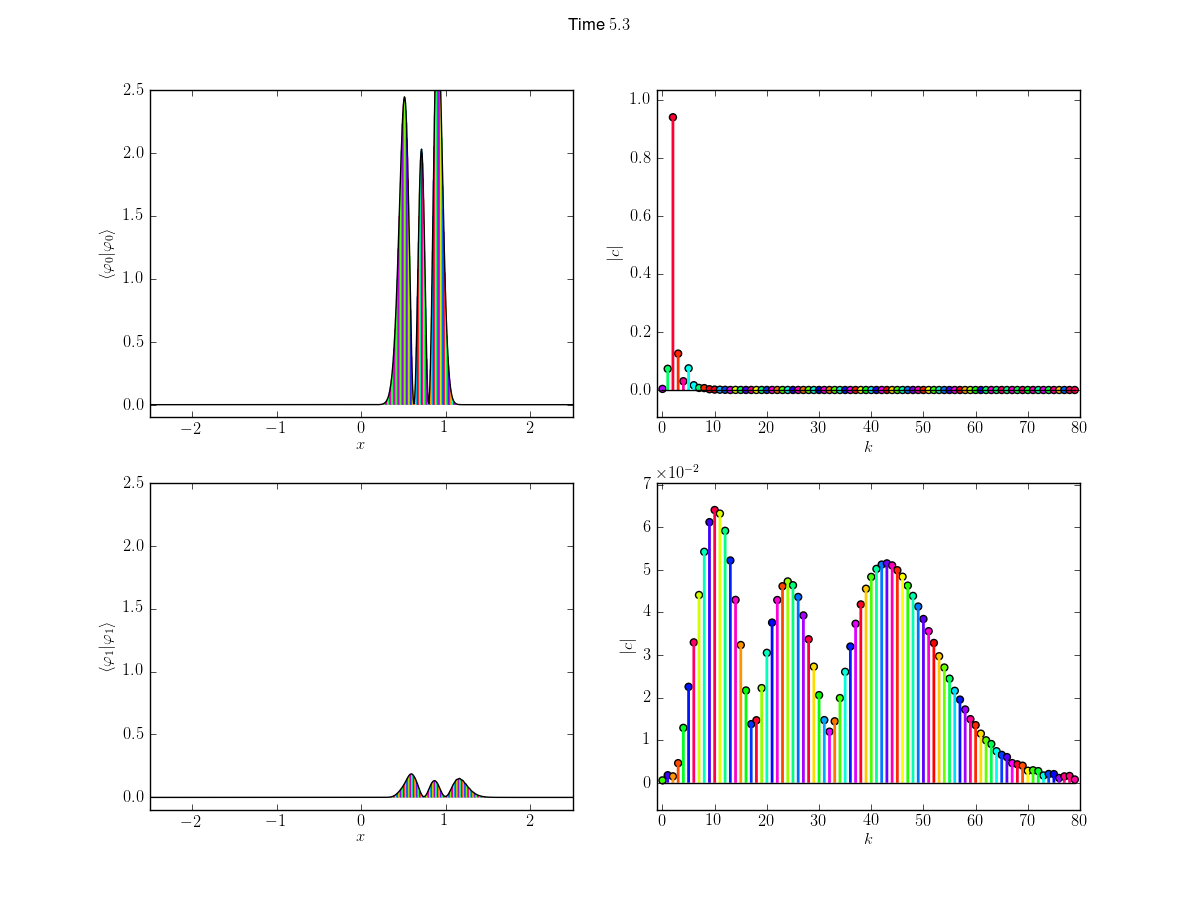
\includegraphics[width=\linewidth]{./figures/spawn_issues_k_na.png}
  \caption[Snapshot of a $\phi_2$ wavepacket in an avoided crossing]{If we spawn
  on the upper level then we can justify to choose $k=2$ but when we would like
  to spawn on the lower level, it is by far not obvious how to choose $k$. One
  could start guessing and try f.e. the median. In both cases the fragment (left
  panels) used for estimating parameters has the shape of a $\phi_2$.}
  \label{fig:spawn_issues_k_na}
\end{figure}

~\newline

The last open issue we would like to mention here is that sometimes the relation

\begin{equation}
  |\tilde{P}|^2 |\tilde{Q}|^2 \geq 1
\end{equation}

is violated. This is really bad because this inequality expresses Heisenberg's
uncertainty principle which is fundamental in quantum physics and should always
be fulfilled, see also \cite[remark 2.7]{H_ladder_operators}. Violations of this
inequality will in turn induce a violation of the compatibility relations \eqref{eq:symplecticity_condition}.

The origin of these problems is again formula \eqref{eq:estimate_abssqrPQ}. The
equation shown there is mathematically only correct for single basis functions
$\phi_k$ and does not provide any solution for linear combinations like our
fragments. Because of this it is strictly speaking not allowed to plug in
the estimated second moments of $w$ as we did. This discrepancy is what
causes the violation of the uncertainty principle. Luckily for us it happened
in the simulations only at times where spawning would make no sense anyway.
And we should add that it never happened if $k=0$ but this is no solution either
as it will hinder the spawning process taking place at times when the
violation is not present.

It's not clear what the best way to proceed from here is. Also it's not clear how
important an accurate guess of $\tilde{P}$ and $\tilde{Q}$ really is. For example
one can obtain a decent result by performing spawning by doing basis projection
and using a large enough target basis.

\end{chapter}
